% Generated in part using

% https://github.com/numpde/ibiocomp/blob/main/code/20201229_LogicalTables/PlayerA.py

% and
	
% https://crcit.net/c/205b0db18f954c4585b3f87d69fced6c
% https://crcit.net/c/84159c89986c4330978603aeace14aa1

% RA, 2020-12-30
	
\begin{table}[hpbt]
	\centering

	\begin{minipage}{0.3\linewidth}
		\centering
				
		Winning strategy:
		
		{\ }
		
		\begin{tabular}{cccc|c}
		\multicolumn{4}{c|}{Sticks left} & Take \\
		\hline
		15 & 11 & 7 & 3 & 2 \\
		14 & 10 & 6 & 2 & 1 \\	
		13 & 9  & 5 & 1 & 1 \\	
		12 & 8  & 4 &   & 3 \\	
		\end{tabular}
	\end{minipage}
	%
	\qquad
	%
	\begin{minipage}{0.25\linewidth}
		\centering
		\begin{tabular}{ccc|cc}
		\cee{w_A} &  \cee{s_1} &  \cee{s_0} &  \cee{r_1} &  \cee{r_0} \\
		\hline
		  0 &   0 &   0 &   0 &   0 \\
		  0 &   0 &   1 &   0 &   0 \\
		  0 &   1 &   0 &   0 &   0 \\
		  0 &   1 &   1 &   0 &   0 \\
		  1 &   0 &   0 &   1 &   1 \\
		  1 &   0 &   1 &   0 &   1 \\
		  1 &   1 &   0 &   0 &   1 \\
		  1 &   1 &   1 &   1 &   0 \\
		\end{tabular}
	\end{minipage}
	%
	\qquad
	%
	\begin{minipage}{0.3\textwidth}
		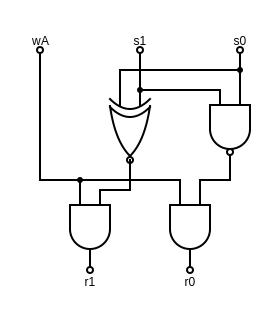
\includegraphics[width=\linewidth]{circuits/Logical-PlayerA}
	\end{minipage}
	
	\caption{%
		Logical circuit for {Player A}.
		%
		The input is a
		wake-up signal \cee{w_A}
		and the bits
		\cee{s_1}/\cee{s_0}
		of the current number of sticks
		(\cee{8 s_3 + 4 s_2 + 2 s_1 + s_0}).
		%
		The output is
		the number of sticks that 
		the player chooses to take,
		encoded as \cee{2 r_1 + r_0}.
		%
		Note that the output is cut off
		when \cee{w_A} is absent.
		%
		%
		The circuit for {Player B}
		is identical except
		that it is controlled up by \cee{w_B}.
	}
	
	\label{t:logical-playera}
\end{table}
